\documentclass[openany,italian,12pt]{article}
\usepackage[letterpaper,top=2cm,bottom=2cm,left=3cm,right=3cm,marginparwidth=1.75cm]{geometry}
\usepackage[utf8]{inputenc}
\usepackage[italian]{babel}
\usepackage[Lenny]{fncychap}
\usepackage{url}
\usepackage{lipsum}
\usepackage{graphicx}
\usepackage[version=4]{mhchem}
\usepackage{amsmath}
\usepackage{mathtools,amsfonts,amssymb}
\usepackage{booktabs}
\usepackage{multirow}
\usepackage{biblatex}
\usepackage{arydshln} % Pacchetto per le linee tratteggiate
\renewcommand{\arraystretch}{1.5}
\usepackage[table]{xcolor} % Pacchetto per colorare celle
\renewcommand{\arraystretch}{1.5}
\usepackage{tikz}
\usetikzlibrary{decorations.markings}
\usetikzlibrary{arrows.meta}
\usepackage{rotating}
\usetikzlibrary{calc}

\newcommand{\tikzmark}[1]{\tikz[overlay,remember picture] \node (#1) {};}

\usepackage{bbold}
\usepackage{booktabs}
\usepackage[arrowdel]{physics}
\usepackage{cancel}
\usepackage{float}
\usepackage{enumitem}
\usepackage{hyperref}
\hypersetup{
    colorlinks,
    citecolor=black,
    filecolor=black,
    linkcolor=black,
    urlcolor=black
}

\usepackage{import}

\makeatletter
\newcommand{\lambdabar}{{\mathchoice
  {\smash@bar\textfont\displaystyle{0.25}{1.2}\lambda}
  {\smash@bar\textfont\textstyle{0.25}{1.2}\lambda}
  {\smash@bar\scriptfont\scriptstyle{0.25}{1.2}\lambda}
  {\smash@bar\scriptscriptfont\scriptscriptstyle{0.25}{1.2}\lambda}
}}
\newcommand{\smash@bar}[4]{%
  \smash{\rlap{\raisebox{-#3\fontdimen5#10}{$\m@th#2\mkern#4mu\mathchar'26$}}}%
}
\makeatother

\newcommand{\A}{\text{Å} \hspace{0.1mm}}

\newcommand{\E}{È \hspace{0.1mm}}

\newcommand\parallelo{/\!/}

\setlength\parindent{0pt}

\DeclareUnicodeCharacter{2212}{-}

\newlist{Properties}{enumerate}{2}
\setlist[Properties]{label=(p.\arabic*),itemindent=*}

\begin{document}

\thispagestyle{empty}
\begin{center}


\uppercase{\sc{ \Large{\textbf{Università degli studi di Torino}}}}\\
\sc{ \large{\textbf{Dipartimento di Fisica}}}\\

\medskip
\hbox to \textwidth{\hrulefill}
\vfill
\uppercase{\sc{ \Large{\textbf{Report }}}}\\
\uppercase{\sc{ \Large{\textbf{Reti Neurali}}}}\\

\vfill


\uppercase{\sc{ \Large{Riconoscimento di segnali stradali}}}\\

\vfill
\begin{center}
    \large{A cura di}
    
    \vspace{0.5cm}
    
    \large{Marco Gorgone}    
\end{center}

\vfill
\vfill
\hbox to \textwidth{\hrulefill}
{\sc anno 2025/2026}
\end{center}

\newpage

\tableofcontents

\newpage

\section{Problema: Riconoscimento dei Segnali Stradali}
In questa era dell'Intelligenza Artificiale, gli esseri umani stanno diventando sempre più dipendenti dalla tecnologia. Con la tecnologia avanzata, aziende multinazionali come Google, Tesla e molte altre stanno lavorando per automatizzare i veicoli, cercando di creare veicoli autonomi o senza conducente il più possibile precisi. Infatti le auto a guida autonoma, in cui il veicolo stesso si comporta come un'autista, non ha bisogno di alcuna guida umana per circolare sulla strada. Non è sbagliato preoccuparsi degli aspetti legati alla sicurezza, in quanto è sempre presente la possibilità di incidenti. Ma sappiamo che nessuna macchina è più precisa degli esseri umani. I ricercatori stanno eseguendo numerosi algoritmi per garantire una sicurezza stradale al 100$\%$. Fra questi, un algoritmo fondamentale è il \textbf{Riconoscimento dei Segnali Stradali}.

Quando si è in strada, si vedono vari segnali stradali come curve a sinistra o a destra, limiti di velocità, divieto di sorpasso ai veicoli pesanti, divieto di accesso, attraversamento pedonale per bambini, ecc., che è necessario seguire per una guida sicura. Allo stesso modo, i veicoli autonomi devono anche interpretare questi segnali e prendere decisioni per garantire la precisione. Per riconoscere a quale categoria appartiene un segnale stradale è necessario quindi classificarli.

In questo progetto di Machine Learning, costruiremo un modello per la classificazione dei segnali stradali presenti nell'immagine in molte categorie utilizzando una rete neurale convoluzionale (CNN).

In figura \ref{Esempio} è presente un esempio visivo che descrive il problema. 
\vspace{+1truecm}
\begin{figure}[H]
    \centering
    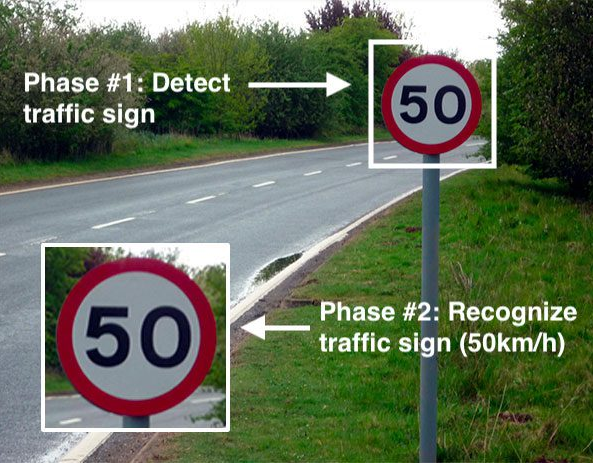
\includegraphics[scale=0.6]{Build/Immagine.png}
    \caption{Esempio}
    \label{Esempio}
\end{figure}

\newpage

\subsection{Dataset}

Il dataset completo delle immagini, scaricabile al link \url{https://www.kaggle.com/datasets/meowmeowmeowmeowmeow/gtsrb-german-traffic-sign}, è composto da più di 50.000 foto di vari segnali stradali (limiti di velocità, attraversamenti, segnali stradali, ecc.), con una dimensione totale di circa 560 MB. \\ Per questo lavoro nello specifico sono state utilizzate le immagini contenute nel percorso\\ $\text{DITS}$, con una dimesione di 450 MB.

\begin{figure}[H]
    \centering
    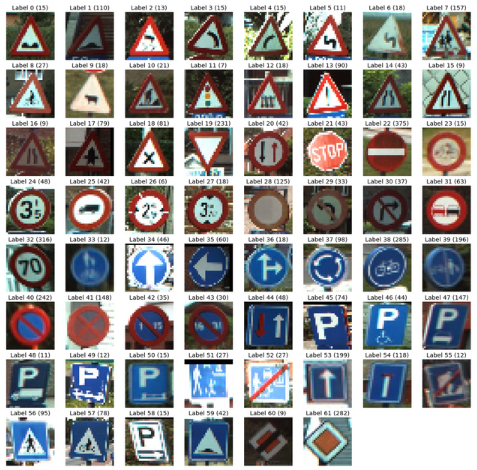
\includegraphics[scale=0.7]{Build/Immagine2.png} 
    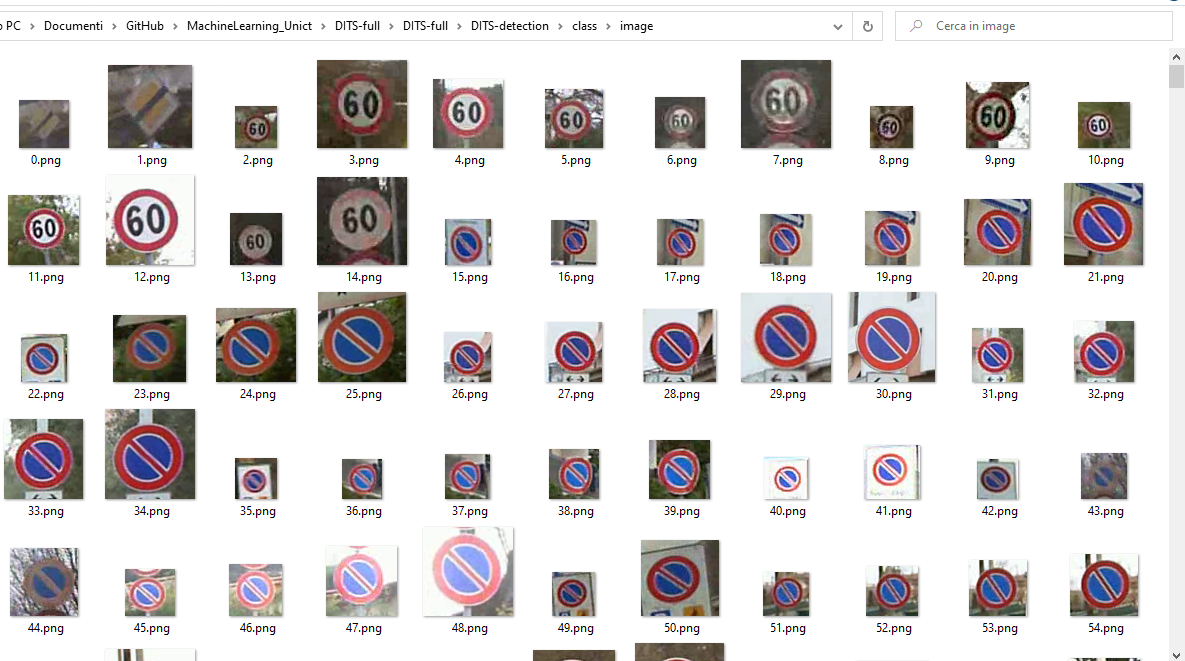
\includegraphics[scale=0.4]{Build/Dataset.png}
    \caption{Esempi visuali dei dati}
    \label{fig:enter-label}
\end{figure}

Del dataset sono presenti due versioni una in cui i segnali sono divisi per segnale specifico e un'ultima da me scelta la divisione per macro categoria di segnale, in questo modo i segnali del dataset si dividono nelle loro 3 macrocategorie, a cui è poi stata aggiunta attraverso uno script una quarta categoria, arrivando ad avere le seguenti categorie:

\begin{itemize}
    \item Divieto
    \item Pericolo
    \item Obbligo    
    \item Backgroud (utile per un secondo scopo)
\end{itemize}

\section{Metodo}

In questa sezione viene descritto l'approccio adottato per risolvere il problema, formulato come task di classificazione in quattro categorie (indicazione, pericolo, divieto, background).

\subsection{Rete Utilizzata}

In seguito a una fase preliminare di sperimentazione (discussa nel capitolo successivo), è stata selezionata una Convolutional Neural Network (CNN) ispirata ad AlexNet, denominata \textit{LeNetColor}. L'architettura è stata progressivamente migliorata mediante l'introduzione di \textit{Batch Normalization} e \textit{Dropout}, al fine di stabilizzare l'addestramento e ridurre il rischio di overfitting. Nel seguito, il modello finale viene indicato come \textbf{MiniAlexNetV2}. La Figura \ref{fig:reti} mostra la rete di partenza (\textit{LeNetColor}) e la sua prima evoluzione (\textit{MiniAlexNet}), mentre la Figura \ref{MiniAlexNetV2} riporta l'architettura finale selezionata.

\begin{figure}[htbp]
\centering
\begin{minipage}[t]{0.50\textwidth}
    \centering
    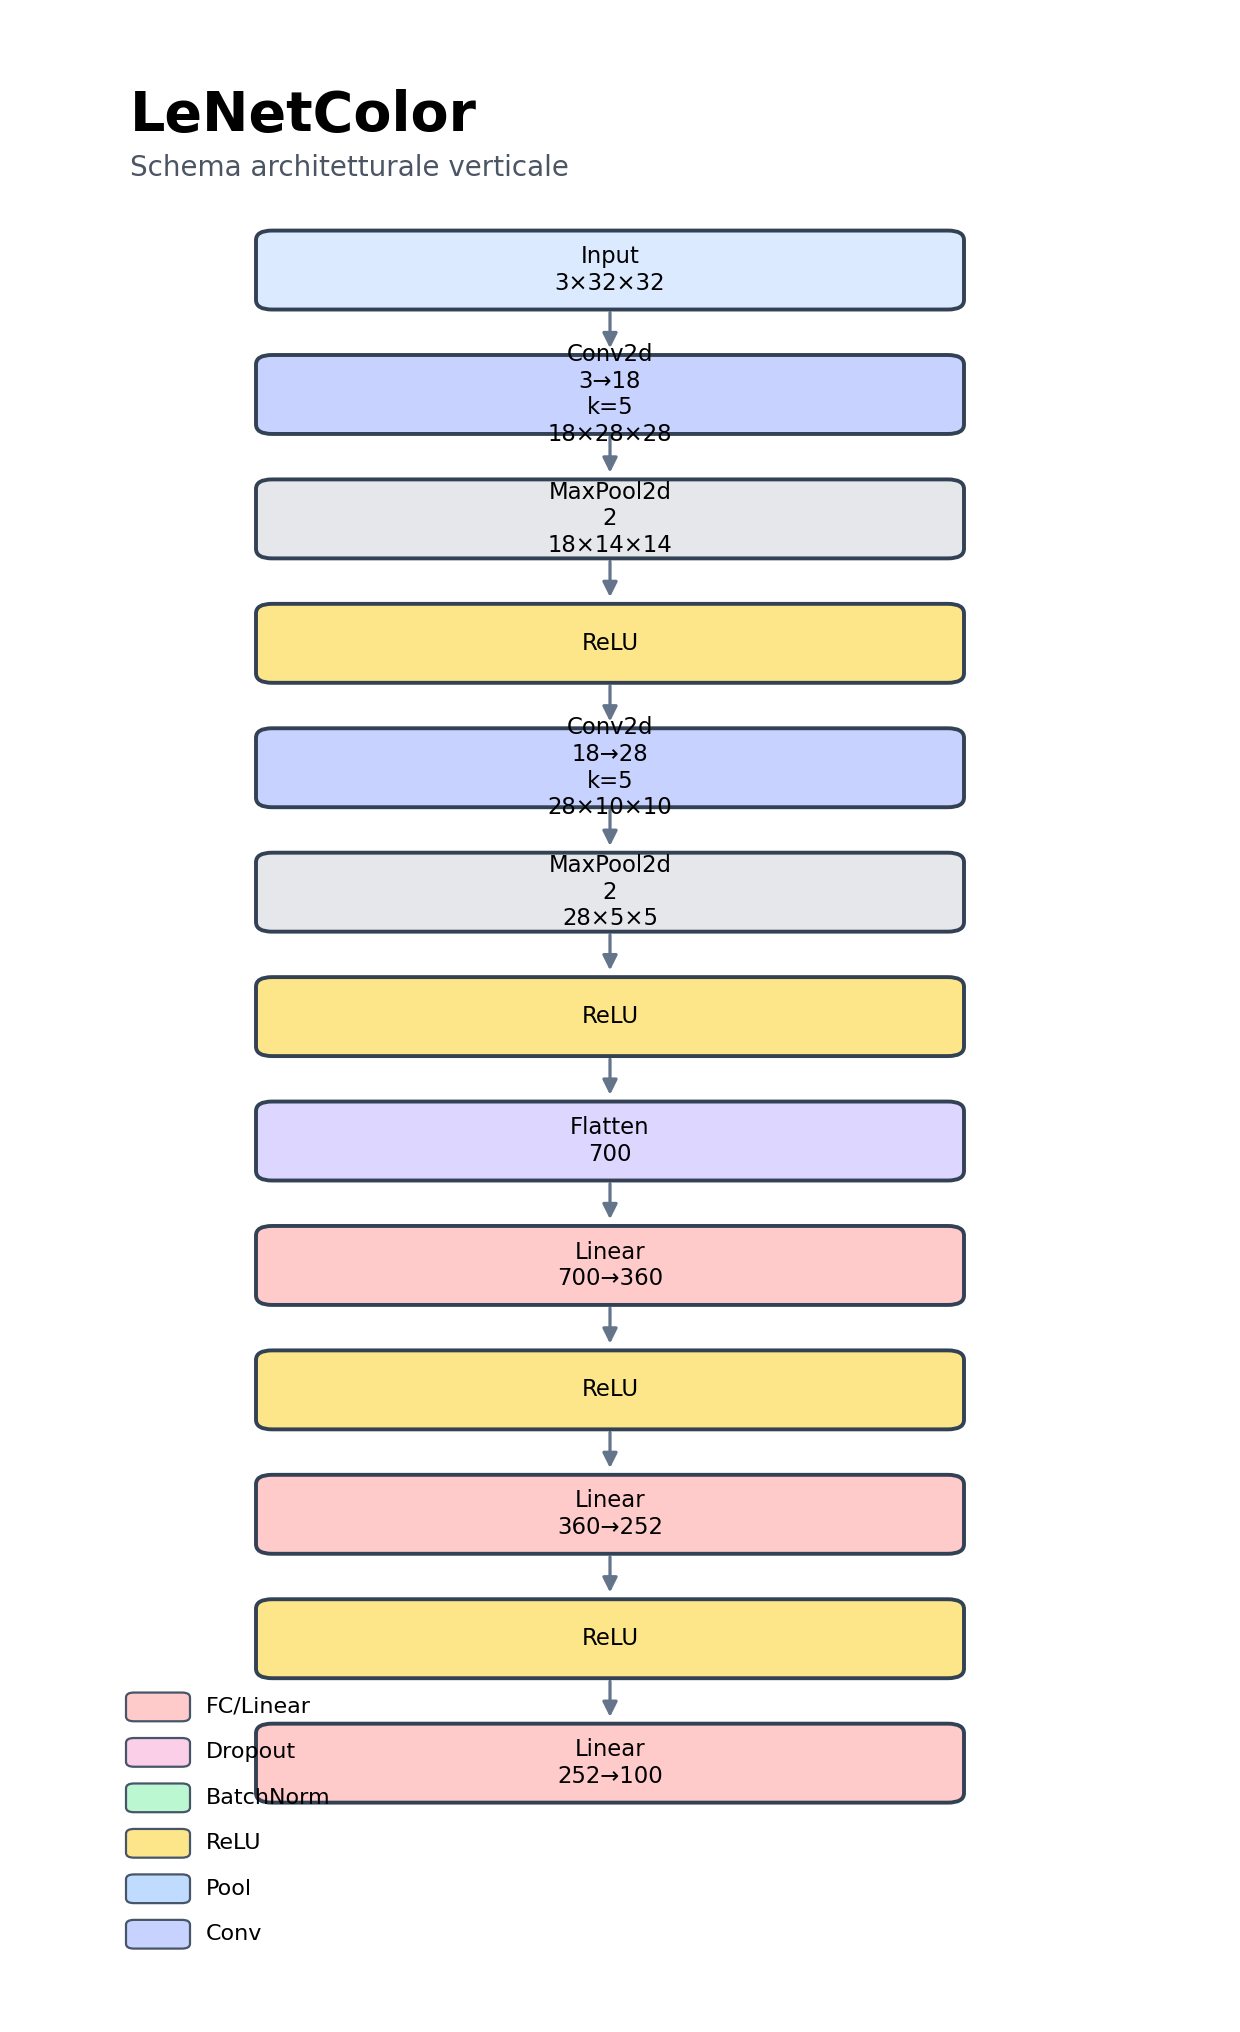
\includegraphics[width=\linewidth]{Metodo/LeNetColor_vertical.png}
\end{minipage}\hfill
\begin{minipage}[t]{0.50\textwidth}
    \centering
    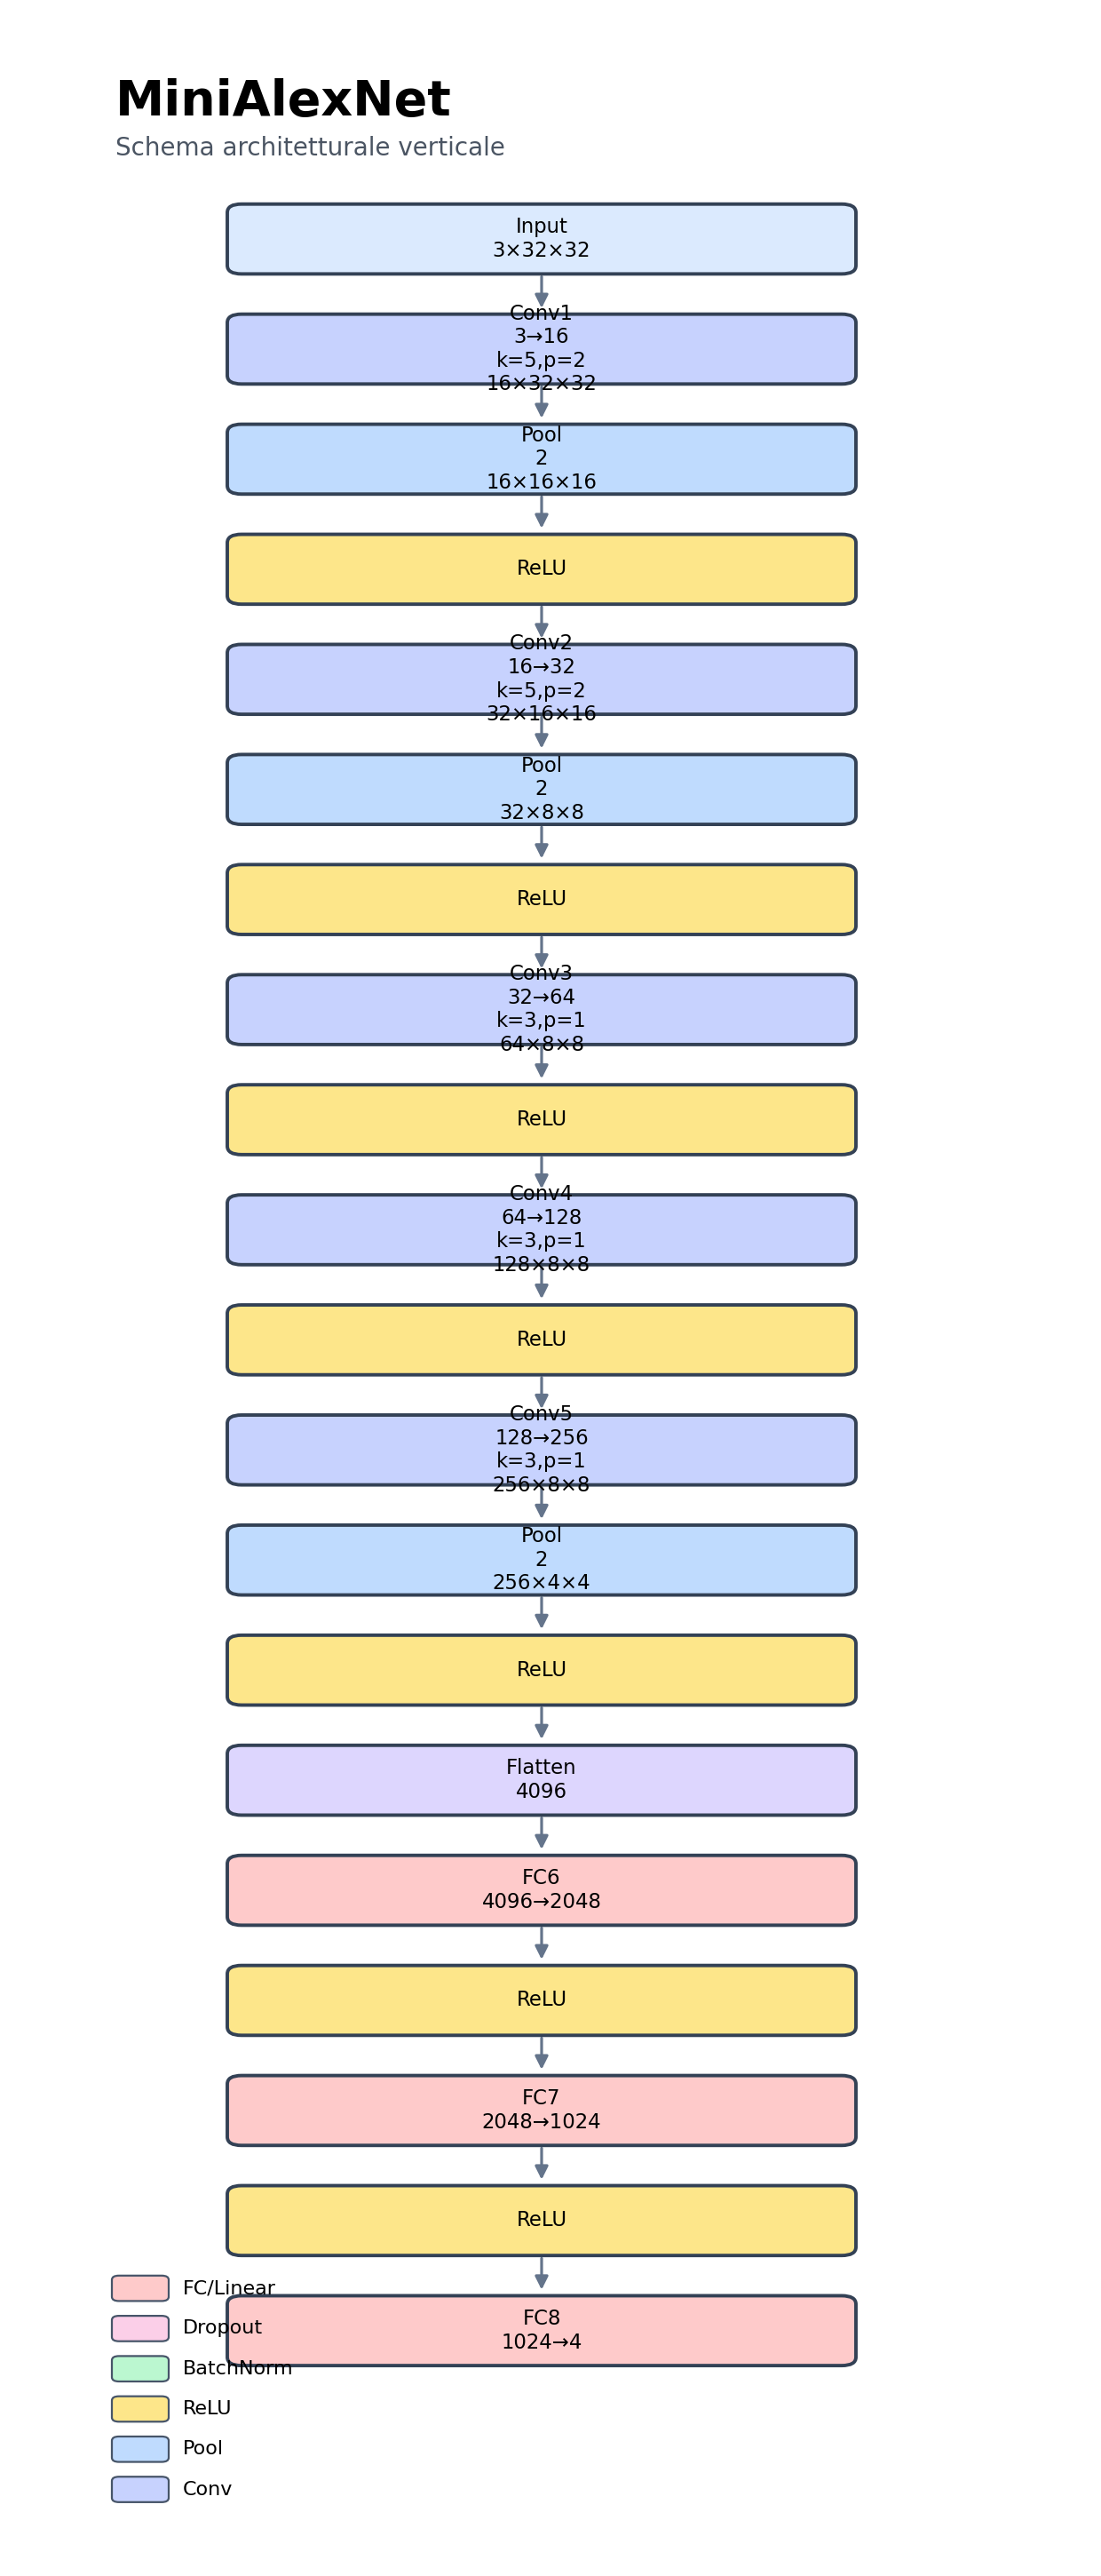
\includegraphics[width=\linewidth]{Metodo/MiniAlexNet_vertical.png}
\end{minipage}\hfill

\caption{Confronto tra LeNetColor e MiniAlexNet}
\label{fig:reti}
\end{figure}

\begin{figure}
    \centering
    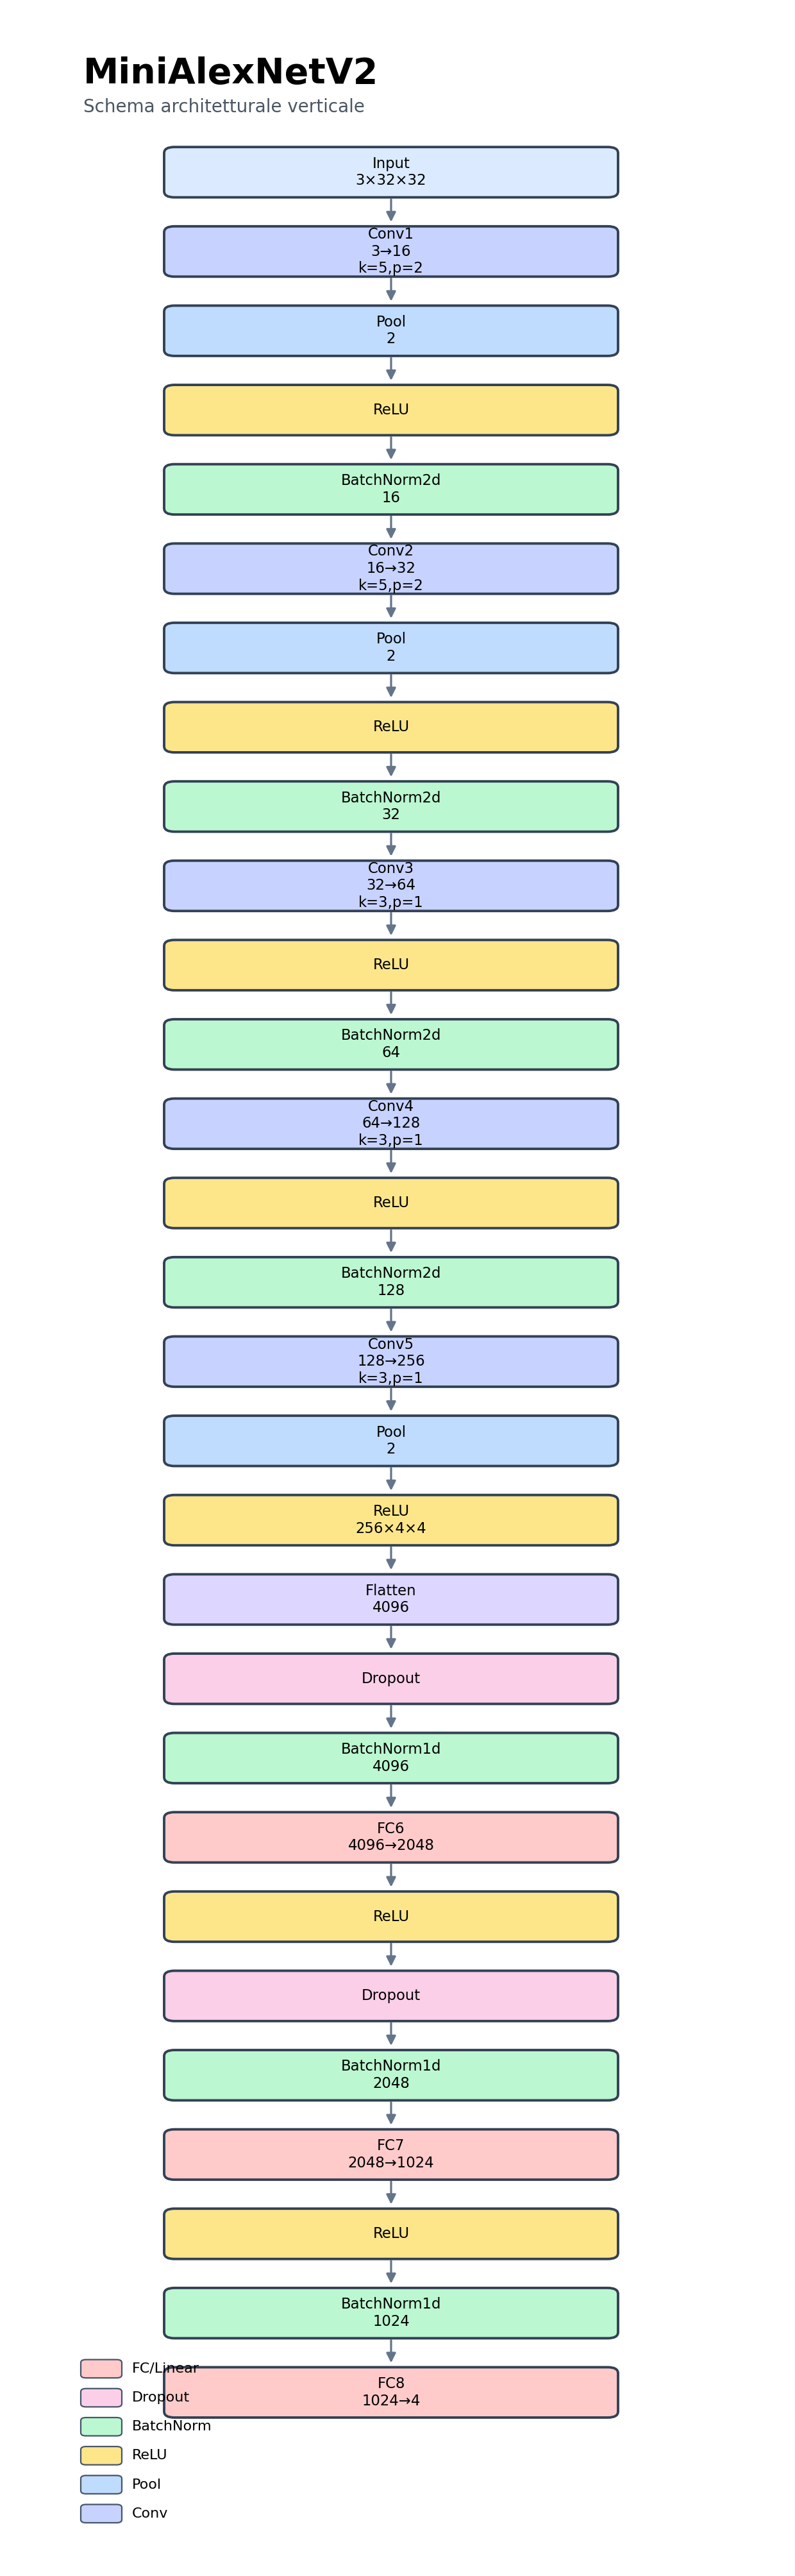
\includegraphics[scale=0.4]{Metodo/MiniAlexNetV2_vertical.png}
    \caption{MiniAlexNetV2, rete utilizzata per il training}
    \label{MiniAlexNetV2}
\end{figure}

Per la configurazione di input sono state adottate scelte empiriche consolidate: batch size pari a 1024 in addestramento e 2048 in validazione/test, con strati di MaxPooling (kernel 2, stride 1). Come funzione di attivazione è stata utilizzata la Rectified Linear Unit (ReLU), che annulla i valori negativi e mantiene invariati i valori positivi. Tale funzione è descritta in \eqref{1}:

\begin{equation}
    f(x) = \begin{cases}
                0 & \text{se } x < 0 \\
                x & \text{se } x > 0
           \end{cases}
\label{1}
\end{equation}

\subsection{Funzione di Loss}
La funzione di loss adottata è la \textit{Cross Entropy Loss}, riportata in \eqref{2}:

\begin{equation}
    \text{Cross Entropy Loss} = -\frac{1}{N} \sum_{i=1}^{N} \sum_{j=1}^{C} y_{ij} \cdot \log(\hat{y}_{ij})
\label{2}
\end{equation}

dove:
\begin{align*}
    N & \text{ è il numero di campioni,} \\
    C & \text{ è il numero di classi,} \\
    y_{ij} & \text{ è la vera probabilità della classe } j \text{ per il campione } i, \\
    \hat{y}_{ij} & \text{ è la probabilità predetta della classe } j \text{ per il campione } i.
\end{align*}

La cross entropy loss consente di confrontare due distribuzioni di probabilità: quella predetta dal modello e quella target. Nel caso in esame, \textbf{MiniAlexNetV2} produce per ciascuna immagine una distribuzione di probabilità sulle classi, che viene confrontata con la distribuzione reale.

In termini operativi, è stata inoltre considerata la seguente variante della funzione di loss:

\begin{equation}
    \text{Cross Entropy Loss} = -\frac{1}{N}\sum_{i}^{N} \left( y_i \cdot \log(\hat{y}_i) + (1 - y_i) \cdot \log(1 - \hat{y}_i) \right)
\label{3}
\end{equation}

dove:
\begin{align*}
    N & \text{ è il numero di classi,} \\
    y_i & \text{ è la vera probabilità della classe } i, \\
    \hat{y}_i & \text{ è la probabilità predetta della classe } i.
\end{align*}

\subsection{Valutazione}
La qualità delle previsioni è stata valutata tramite il parametro di accuratezza, derivato a partire da una matrice di confusione elementare (Tabella \ref{tab:matrice-confusione}):

\begin{table}[H]
\centering
\begin{tabular}{|c|c|c|}
\hline
\multirow{2}{*}{} & \multicolumn{2}{c|}{\cellcolor{gray!20}\textbf{Realtà}} \\ \cline{2-3}
 & \cellcolor{gray!20}\textbf{Positivo} & \cellcolor{gray!20}\textbf{Negativo} \\ \cline{1-3}
\cellcolor{gray!20}\textbf{Previsione Positiva} & \cellcolor{green!20}Vero Positivo & \cellcolor{red!20}Falso Positivo \\ \cline{1-3}
\cellcolor{gray!20}\textbf{Previsione Negativa} & \cellcolor{red!20}Falso Negativo & \cellcolor{green!20}Vero Negativo \\ \cline{1-3}
\end{tabular}
\caption{Matrice di Confusione}
\label{tab:matrice-confusione}
\end{table}

\vspace{+1truecm}

L'accuratezza del modello è definita come rapporto tra il numero di previsioni corrette e il numero totale di previsioni, come espresso in \eqref{4}:
\begin{equation}
\text{Accuracy} = \frac{\text{Numero di Previsioni Corrette}}{\text{Numero Totale di Previsioni}}
\label{4}
\end{equation} 
\newline

Tale parametro fornisce una misura sintetica della capacità di classificazione del modello.
\newline 
Accanto all'accuratezza è stata analizzata anche la curva ROC, che descrive l'andamento delle prestazioni al variare della soglia decisionale.








\section{Analisi}
Inizialmente sono state condotte una serie di analisi allo scopo principale di identificare il modello che ha restituito i risultati più promettenti. Successivamente, ci si è dedicati all'indagine delle configurazioni ottimali del momento, al fine di massimizzare l'accuratezza.
\subsection{Scelta del Modello}
Per identificare il modello ottimale, sono stati condotti diversi approfondimenti. Per il primo approfondimento è stata impiegata una rete nota come \textbf{LeNetColor}, successivamente una rete basata su AlexNet, denominata \textbf{MiniAlexNet}, ed infine, dopo aver introdotto sia layer di Dropout che layer di Batch Normalization, abbiamo ottenuto la versione \textbf{MiniAlexNetV2}. 

\begin{figure}[htbp]
\centering
\begin{minipage}[t]{0.33\textwidth}
    \centering
    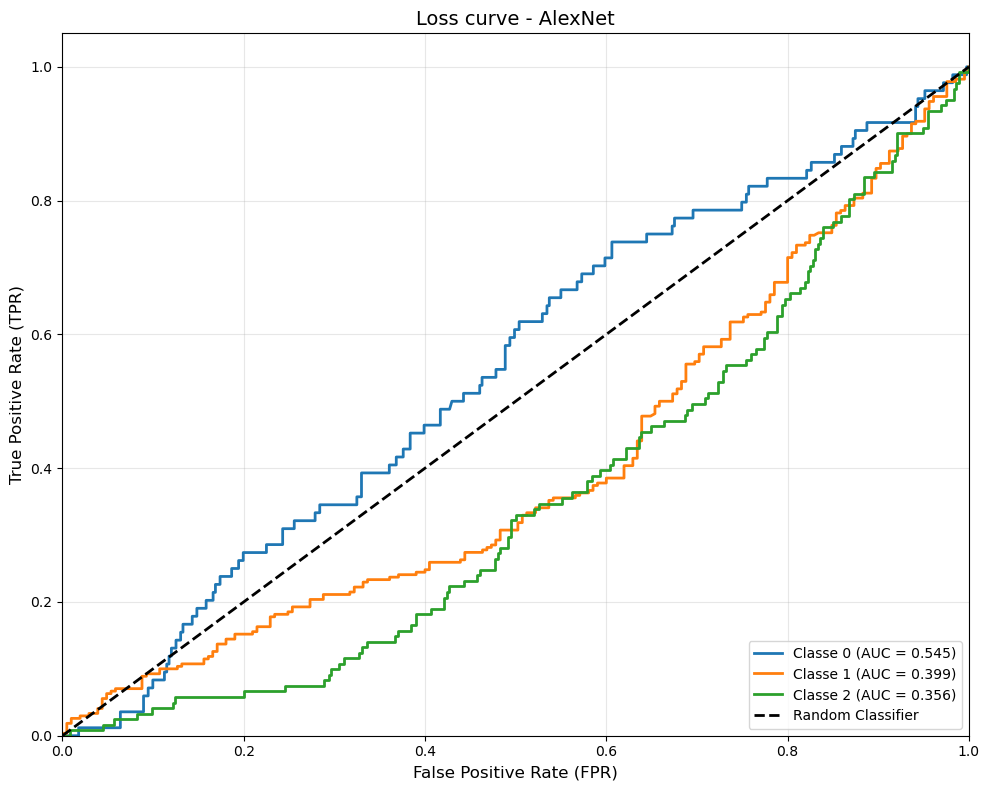
\includegraphics[width=\linewidth]{Analisi/LeNetColor_ROC.png}
\end{minipage}\hfill
\begin{minipage}[t]{0.34\textwidth}
    \centering
    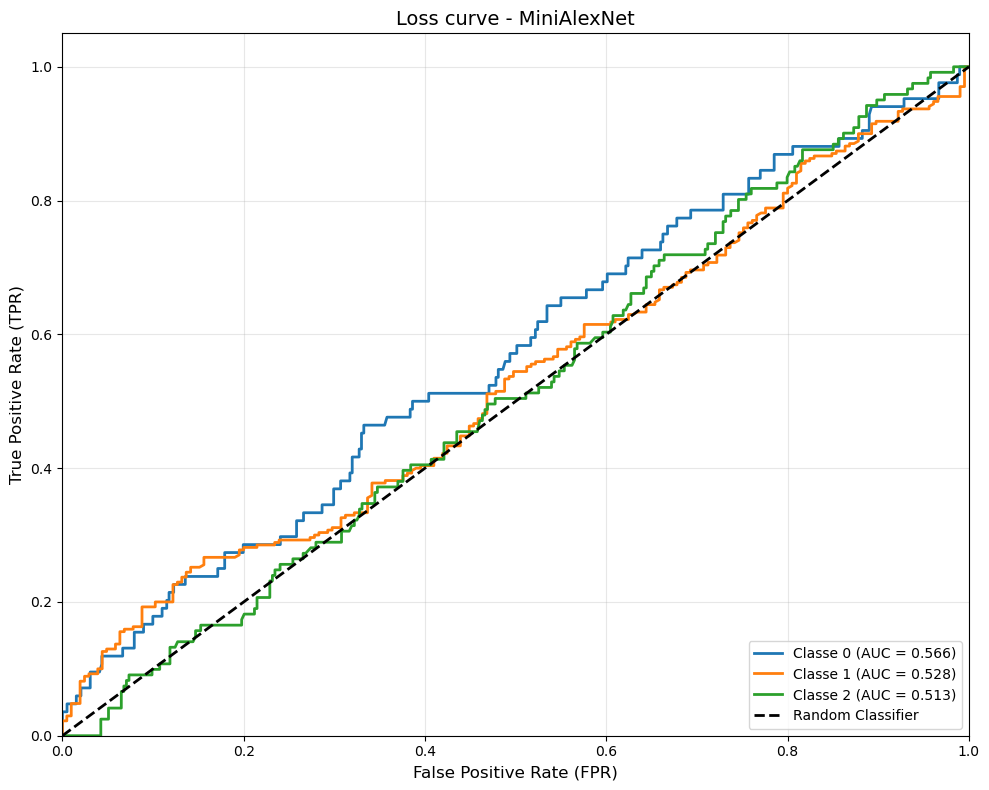
\includegraphics[width=\linewidth]{Analisi/MiniAlexNet_ROC.png}
\end{minipage}\hfill
\begin{minipage}[t]{0.33\textwidth}
    \centering
    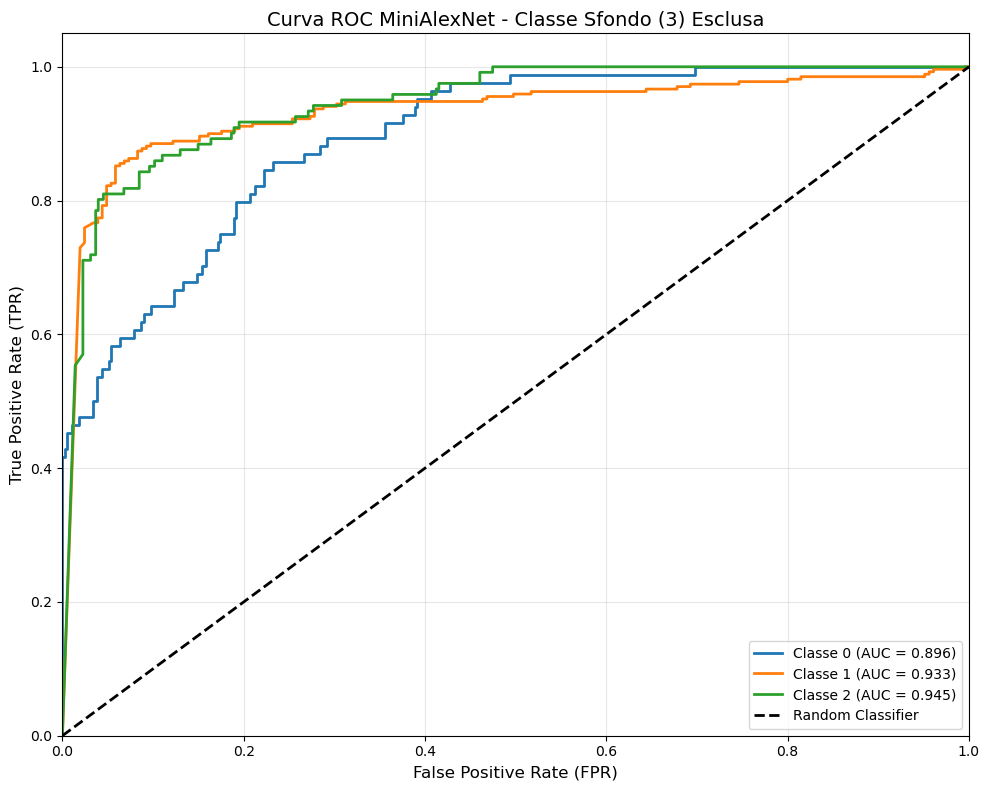
\includegraphics[width=\linewidth]{Analisi/MiniAlexNetV2_ROC.png}
\end{minipage}\hfill

\caption{Confronto tra le ROC curve delle tre reti}
\label{fig:Roc}
\end{figure}

L'esame della Figura  \ref{fig:Roc} evidenzia in modo netto come la rete MiniAlexNetV2 raggiunga un'accuratezza notevolmente superiore rispetto alla MiniAlexNet, che mostra, al contrario, un comportamento oscillante. Sebbene la AlexNet presenti un andamento migliore rispetto alla MiniAlexNet, essa rimane comunque inferiore alla MiniAlexNetV2. Pertanto, dal punto di vista dell'accuratezza, la rete MiniAlexNetV2 emerge come la più efficace.

\begin{figure}[H]
    \centering
    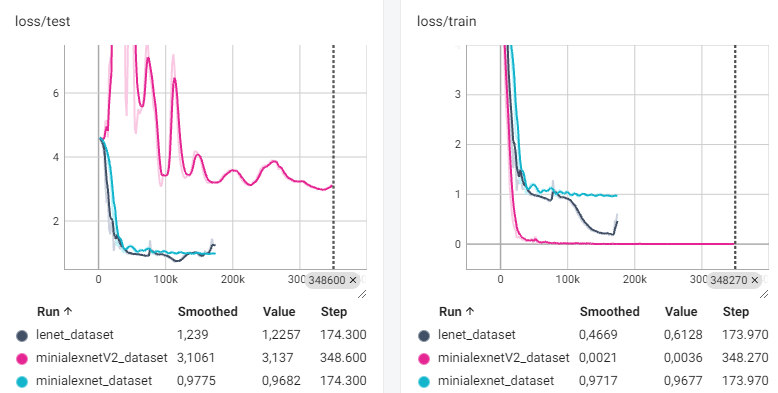
\includegraphics[scale=0.8]{Analisi/ConfrontoLoss.png}
    \caption{Comparazione tra curve loss}
    \label{ConfrontoLoss}
\end{figure}

Dall'analisi della Figura \ref{ConfrontoLoss}, emergono notevoli differenze tra le reti MiniAlexNetV2, MiniAlexNet, e AlexNet, le quali sono state addestrate rispettivamente per 200 epoche durante la fase di training. La rete MiniAlexNetV2 mostra valori di loss inferiori rispetto alle altre due reti.

Tuttavia, durante la fase di test, la curva della MiniAlexNetV2 mostra inizialmente un picco, indicativo di una probabile fase di overfitting nelle prime epoche. Successivamente, la curva si stabilizza su valori di loss più contenuti. Questo comportamento sottolinea la complessità dell'addestramento e la necessità di valutare attentamente le dinamiche della loss durante l'intero processo di addestramento e test. \\
Questi risultati hanno indotto la concentrazione degli sforzi sull'ulteriore sviluppo della rete MiniAlexNetV2. \\
I parametri utilizzati per queste prove sono stati:

\begin{itemize}
  \item Tasso di apprendimento (\textit{Learning Rate}): 0.0001
  \item Momento (\textit{Momentum}): 0.6
\end{itemize}

\subsection{ROC Curve}
Trovati quindi modello e momento, come mostrato prima, è stato reiterato il processo di training, allenando le reti per altre 200 epoche e calcolando la ROC Curve, come mostrato in Figura \ref{fig:Roc}. La curva ROC, che rappresenta la relazione tra il tasso di veri positivi (TPR) e il tasso di falsi positivi (FPR) al variare della soglia di classificazione, è stata utilizzata per valutare le prestazioni del modello in modo più dettagliato.

\begin{figure}[htbp]
\centering
\begin{minipage}[t]{0.33\textwidth}
    \centering
    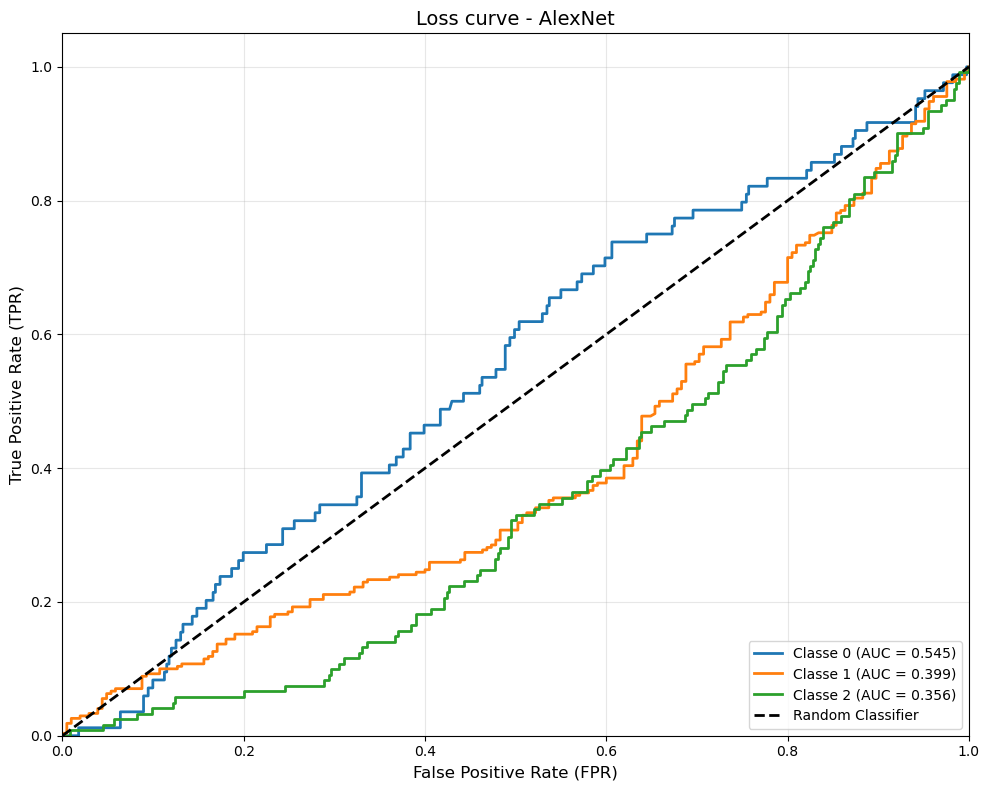
\includegraphics[width=\linewidth]{Analisi/LeNetColor_ROC.png}
\end{minipage}\hfill
\begin{minipage}[t]{0.34\textwidth}
    \centering
    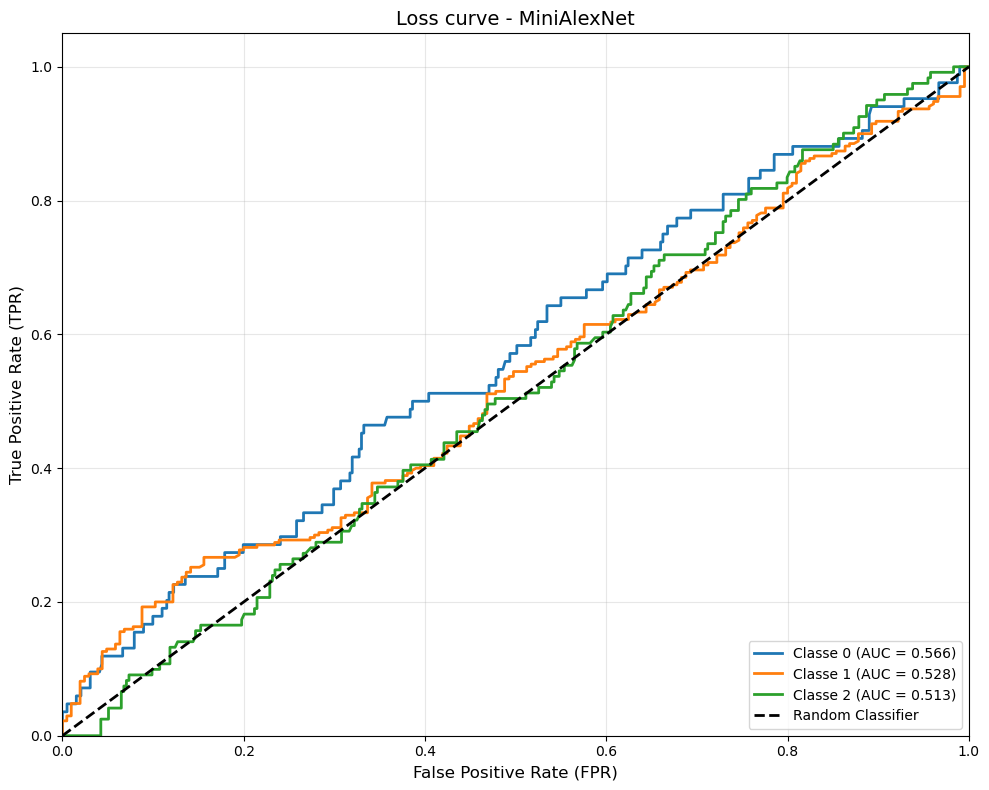
\includegraphics[width=\linewidth]{Analisi/MiniAlexNet_ROC.png}
\end{minipage}\hfill
\begin{minipage}[t]{0.33\textwidth}
    \centering
    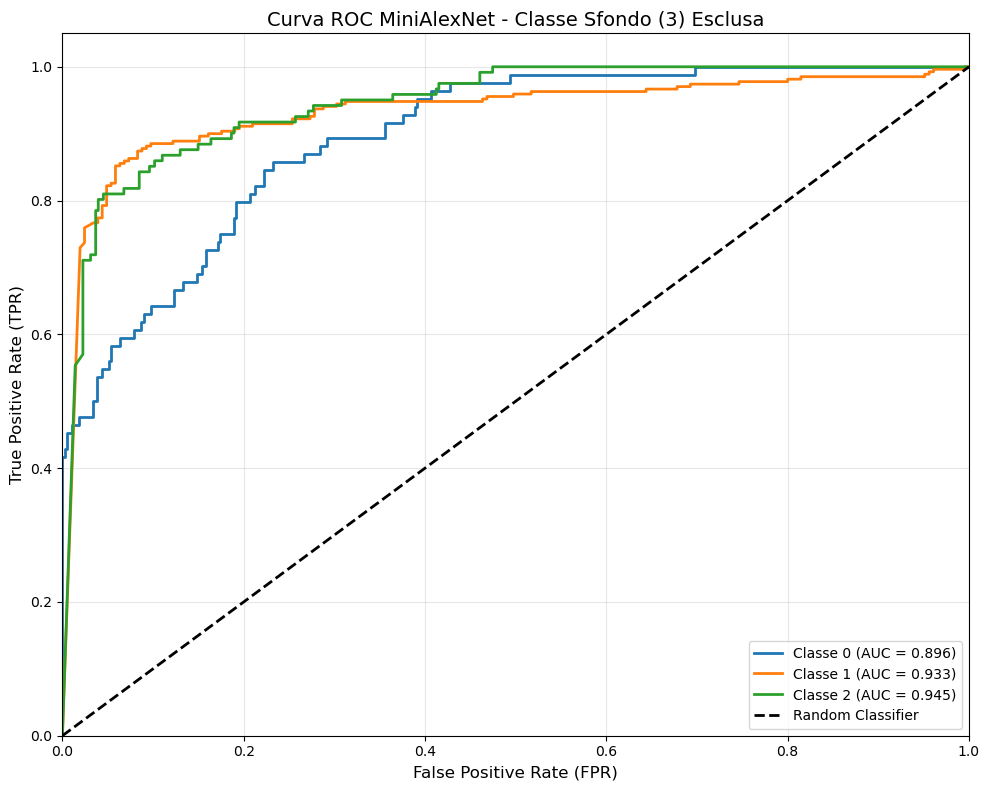
\includegraphics[width=\linewidth]{Analisi/MiniAlexNetV2_ROC.png}
\end{minipage}\hfill

\caption{Confronto tra le ROC curve delle tre reti}
\label{fig:Roc}
\end{figure}

\newpage 

\subsection{Calibrazione del Momento}
Una volta definito il modello, sono stati dedicati sforzi all'ottimizzazione del momento al fine di calibrarlo al meglio. Per valutare l'efficacia di diverse opzioni di momento, ho considerato solo quale tra i valori proposti conducesse a un aumento dell'accuratezza congiuntamente a una convergenza della loss verso valori inferiori.

I dati sull'accuratezza e sulla loss durante l'addestramento del precedente esperimento con MiniAlexNetV2 sono stati conservati. Successivamente, la rete è stata nuovamente addestrata utilizzando un valore di momento pari a 0.7.
I risultati di questo test sono illustrati nella Figura \ref{ConfrontoCurve}. \\ Come evidenziato, il modello presenta un'accuratezza leggermente superiore durante la fase di addestramento e test quando il momento è impostato a 0.6. Le curve di loss convergono a valori leggermente inferiori e seguono un andamento poco più regolare.

Sulla base di tali risultati, si è proceduto mantenendo un valore di momento pari a 0.6.
 
\begin{figure}[H]
    \centering
    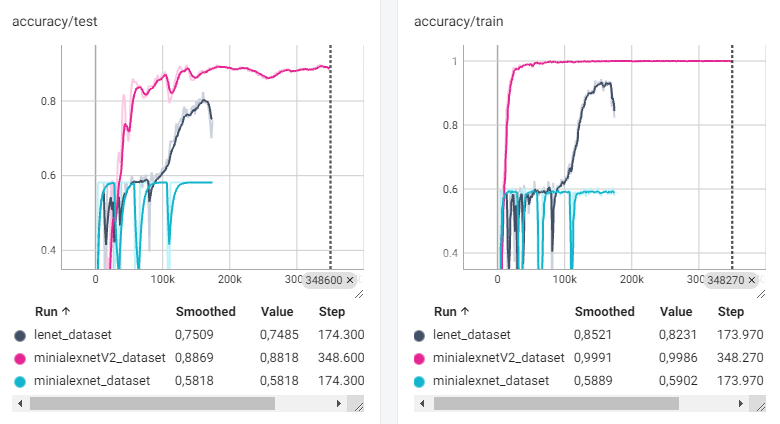
\includegraphics[scale=0.7]{Analisi/ConfrontoAccuracySmooth0.7.png}
    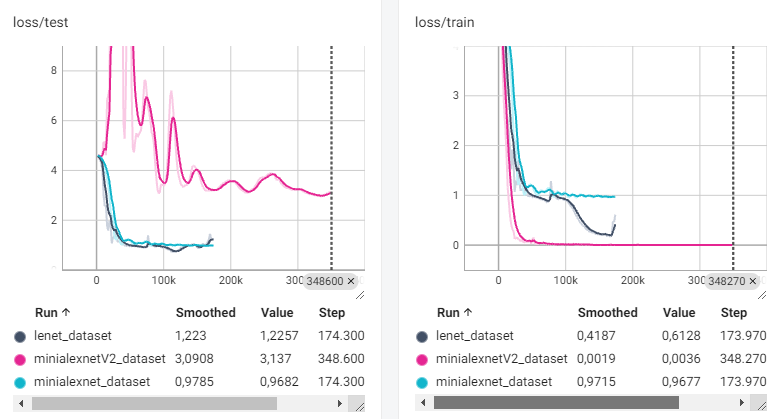
\includegraphics[scale=0.7]{Analisi/ConfrontoLossSmooth0.7.png}
    \caption{Comparazione tra curve accuracy sopra, tra curve loss sotto.}
    \label{ConfrontoCurve}
\end{figure}
\newpage

\section{Codice}
Il codice del progetto è stato organizzato nella sottocartella \texttt{python\_file}, che contiene i seguenti moduli:
\begin{itemize}
    \item Il file \texttt{dataclass} definisce le classi e le trasformazioni per la gestione del dataset di segnali stradali. In particolare, include le classi per l'addestramento (\texttt{StreetSignDataset}) e per il test (\texttt{StreetSignTest}), oltre a trasformazioni quali ridimensionamento (\texttt{Rescale}), ritaglio casuale (\texttt{RandomCrop}), ritaglio specifico (\texttt{Crop}) e conversione in tensori (\texttt{ToTensor}). È inoltre presente la funzione \texttt{show\_landmarks\_batch}, utilizzata per visualizzare batch di immagini con i relativi \textit{landmarks}. Nel complesso, il modulo fornisce l'infrastruttura necessaria alla preparazione dei dati.
    \item Il file \texttt{function} raccoglie le funzioni principali per addestramento e test del classificatore. La prima parte del codice esegue l'addestramento mediante \textit{Stochastic Gradient Descent} e \textit{Cross Entropy Loss}, con supporto a TensorBoard e salvataggio dei pesi. La seconda parte valuta il modello sul set di test, restituendo predizioni ed etichette reali. Nello stesso file sono inoltre presenti le funzioni per l'esportazione dei risultati in formato JSON/CSV e per la generazione dei grafici di accuratezza e loss. È infine inclusa una funzione per il calcolo e la visualizzazione della curva ROC a partire da etichette e predizioni.
    \item Il file \texttt{network} implementa le architetture di rete neurale testate, includendo diverse varianti e l'impiego di tecniche quali \textit{Batch Normalization} e \textit{Dropout}, utili a migliorare prestazioni e capacità di generalizzazione.
    \item Il file \texttt{detect\_and\_classify} implementa la procedura per applicare YOLO al riconoscimento dei segnali stradali in immagini di scenario reale. L'immagine viene inizialmente analizzata da YOLO (addestrato su immagini reali) per individuare il segnale; la porzione ritagliata viene quindi fornita alla rete \textbf{MiniAlexNetV2} per la classificazione. Il sistema realizza così una pipeline completa di \textit{detection} e \textit{classification}.
\end{itemize}

Infine, sono stati creati alcuni notebook in Jupyter, nei quali è stata utilizzata la struttura dati definita in precedenza insieme alle funzioni di training e test, al fine di addestrare il modello. Prima dell'addestramento, le immagini vengono convertite nel formato richiesto dalla struttura dati e sottoposte alle opportune trasformazioni. I notebook realizzati sono i seguenti:
\begin{itemize}
    \item I notebook con intestazione \textit{train} si occupano dell'addestramento delle reti \textit{AlexNet}, \textit{MiniAlexNet} e \textit{MiniAlexNetV2}. In particolare, il notebook esegue il caricamento delle immagini, la loro conversione in tensori e l'addestramento dei modelli, salvando i dati di accuratezza e loss per ogni epoca. Al termine dell'addestramento, i pesi dei modelli vengono salvati per essere successivamente utilizzati nei notebook di \textit{test}, \textit{result} e \textit{graphs}.
    \item \textit{graphs}: carica i dati di accuratezza e loss salvati nei notebook di addestramento e genera i grafici corrispondenti (Loss, Accuracy e ROC).
    \item \textit{result}: carica i tre modelli precedentemente addestrati ed esegue una previsione a partire da un'immagine fornita tramite URL oppure da un'immagine locale. Il notebook restituisce quindi la classe predetta del segnale stradale, tra cui \textit{indicatory} (indicazione), \textit{prohibitory} (divieto) e \textit{warning} (pericolo). In caso di errore nella previsione, viene visualizzato il messaggio \textit{ERROR 404 NOT FOUND}. La classe \textit{Background}, sebbene presente nella fase di addestramento, non viene considerata in quanto non rilevante ai fini dell'applicazione.
    \item \textit{test\_reale}: carica esclusivamente il modello \textit{MiniAlexNetV2} e lo utilizza per eseguire la previsione della categoria del segnale stradale presente in un'immagine reale. In questo caso, l'immagine viene prima elaborata per individuare e ritagliare il segnale stradale, che viene successivamente passato alla rete \textit{MiniAlexNetV2} per la classificazione. La classe predetta viene quindi sovrapposta all'immagine, che viene infine visualizzata.
\end{itemize}

\subsection{Caso Reale}
Analizziamo più in dettaglio il notebook \textit{test\_reale} in cui è presente la parte di codice relativa al test della rete neurale in un contesto urbano. Se, per esempio, dotassimo un veicolo di una telecamera per riprendere la strada in tempo reale, potremmo acquisire delle immagini durante il tragitto e verificare la presenza di segnali stradali, inviando infine l'output al sistema di bordo o al guidatore. Per fare ciò, ci si è posti il problema di come isolare la singola immagine del segnale rispetto al contesto. Per eseguire questa ricerca sono stati studiati due processi:

\begin{itemize}
    \item \textbf{Divisione in sottoimmagini:} consiste nel suddividere l'immagine in numerose porzioni e verificare per ognuna di esse se contiene un segnale stradale.
    \item \textbf{Uso di YOLO:} utilizzo di uno strumento di object detection che permette di individuare le regioni d'interesse (ROI) all'interno delle immagini, identificando le porzioni candidate alla classificazione.
\end{itemize}

\subsubsection{Divisione}
L'uso della divisione in sottoimmagini è la soluzione più semplice, ma ha presentato scarsi risultati sia in termini di prestazioni che di affidabilità. Il motivo risiede nella necessità di processare sequenzialmente ogni ritaglio, causando lentezza di calcolo. Inoltre, l'accuratezza è limitata dal fatto che il dataset di addestramento non copre tutte le possibili variazioni del contesto circostante. Si aggiunge poi il problema del ritaglio: quando si esegue il taglio dell'immagine, il segnale non sempre ricade al centro della sottoimmagine e può risultare solo parziale. Questo fa sì che la rete non sia in grado di riconoscere il segnale oppure produca falsi positivi.

\subsubsection{YOLO}
Per ovviare ai limiti della suddivisione manuale, nel notebook \textit{test\_reale} è stato implementato l'uso dell'algoritmo \textbf{YOLO} (You Only Look Once). A differenza dell'approccio precedente, YOLO esegue l'object detection in un unico passaggio, identificando istantaneamente le coordinate dei segnali stradali (\textit{Bounding Boxes}) all'interno di scene complesse, per poi passare la porzione d'immagine ritagliata contenente il segnale alla rete \textit{MiniAlexNetV2} per identificarne la tipologia.

Il flusso di lavoro implementato prevede i seguenti passaggi:
\begin{enumerate}
    \item Caricamento dell'immagine ad alta risoluzione catturata nel contesto urbano.
    \item Applicazione del modello YOLO per individuare le regioni d'interesse (ROI) corrispondenti ai segnali.
    \item Ritaglio (\textit{cropping}) automatico delle aree individuate.
    \item Passaggio dei ritagli alla rete \textbf{MiniAlexNetV2} per la classificazione finale della macro-categoria.
\end{enumerate}

Questo approccio ibrido ha permesso di ottenere una precisione estremamente elevata, poiché la rete di classificazione lavora solo su porzioni di immagine già identificate come "segnali", eliminando il rumore di fondo del contesto cittadino e riducendo drasticamente i tempi di calcolo rispetto alla scansione sequenziale.

\subsubsection{Analisi dei Risultati}
Una volta spiegati i vari metodi, si procede a visualizzare la differenza tra i due approcci utilizzati. Prima nel caso di utilizzo di un'immagine presa dalle immagini di test (Figura \ref{fig:test1}) con cui abbiamo addestrato la rete: possiamo notare che, nel caso dell'algoritmo di \textbf{divisione}, abbiamo ottenuto dei falsi positivi e, inoltre, alcune porzioni di immagine, essendo state ritagliate in modo non perfetto, sono state classificate erroneamente. Per quanto riguarda l'uso di \textbf{YOLO}, invece, si è avuta l'identificazione di un solo segnale, che è stato poi classificato correttamente dalla rete \textit{MiniAlexNetV2}, ma non ha identificato gli altri segnali presenti.

\begin{figure}[htbp]
\centering
\begin{subfigure}[t]{0.50\textwidth}
    \centering
    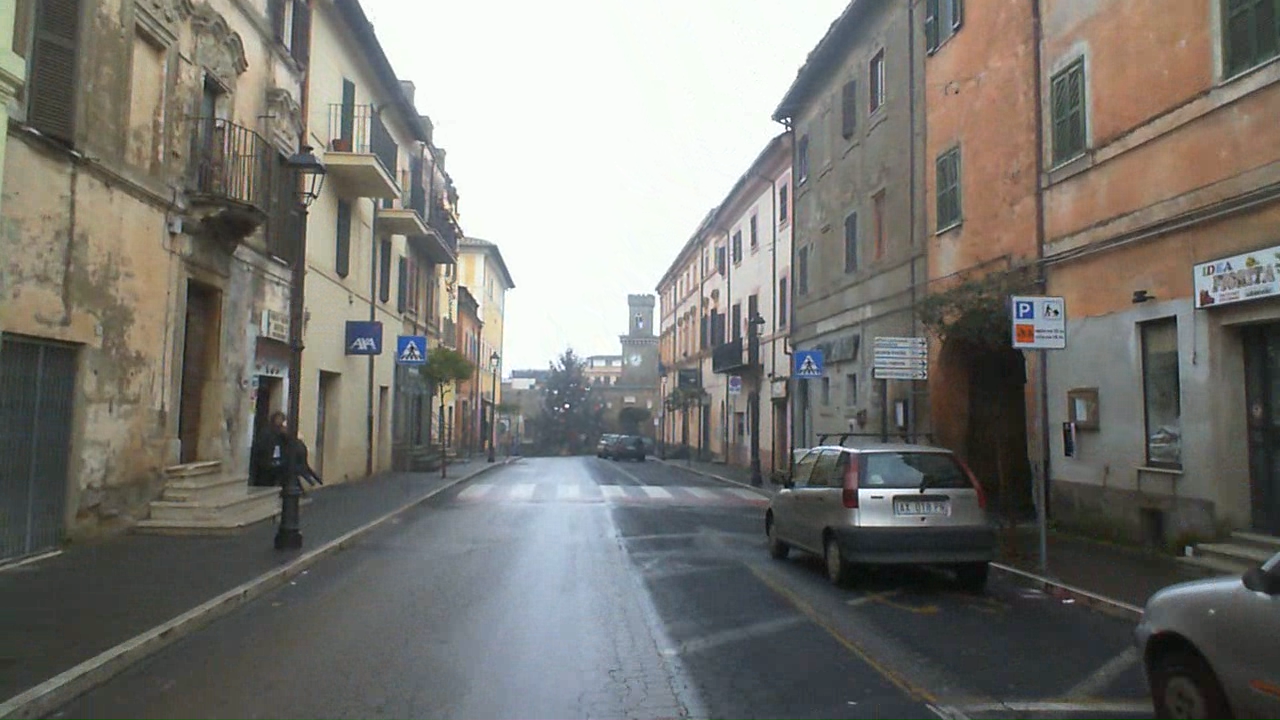
\includegraphics[width=0.9\linewidth]{Codice/test2.png}
    \caption{Immagine originale}
\end{subfigure}\hfill
\begin{subfigure}[t]{0.50\textwidth}
    \centering
    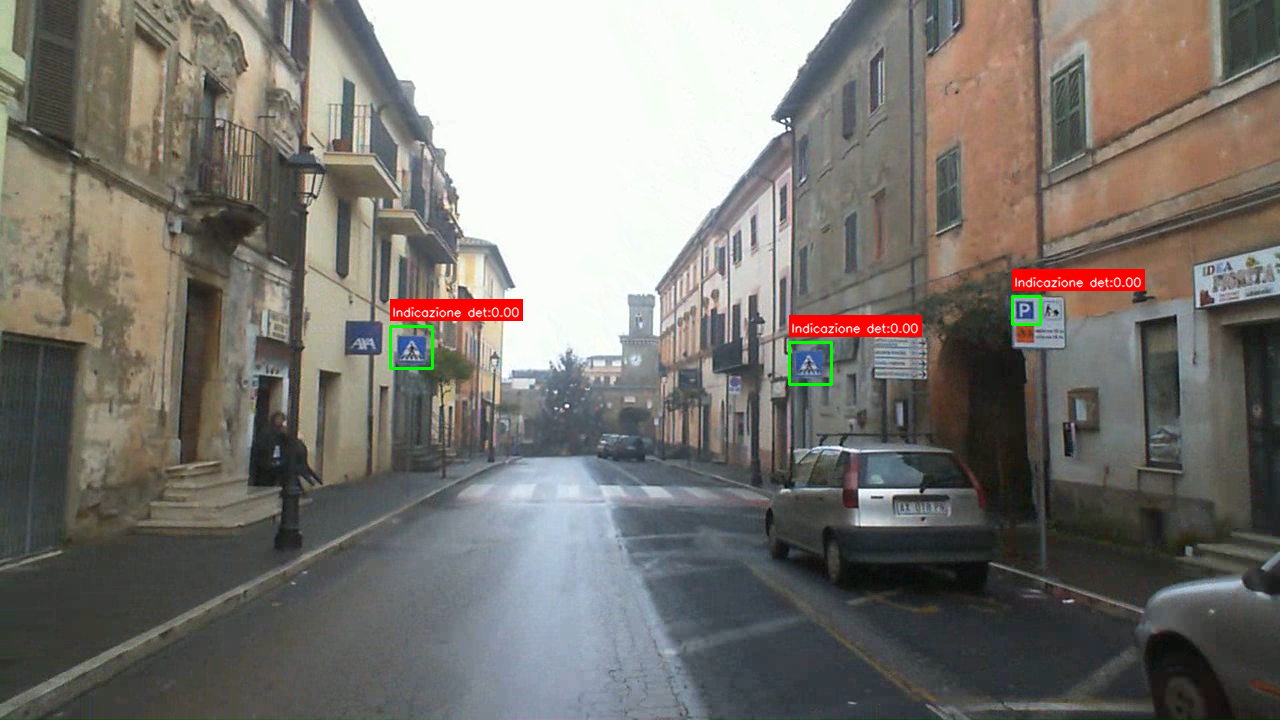
\includegraphics[width=0.9\linewidth]{Codice/test2_std.png}
    \caption{Immagine originale con label}
\end{subfigure}
\vfill
\begin{subfigure}[t]{0.50\textwidth}
    \centering
    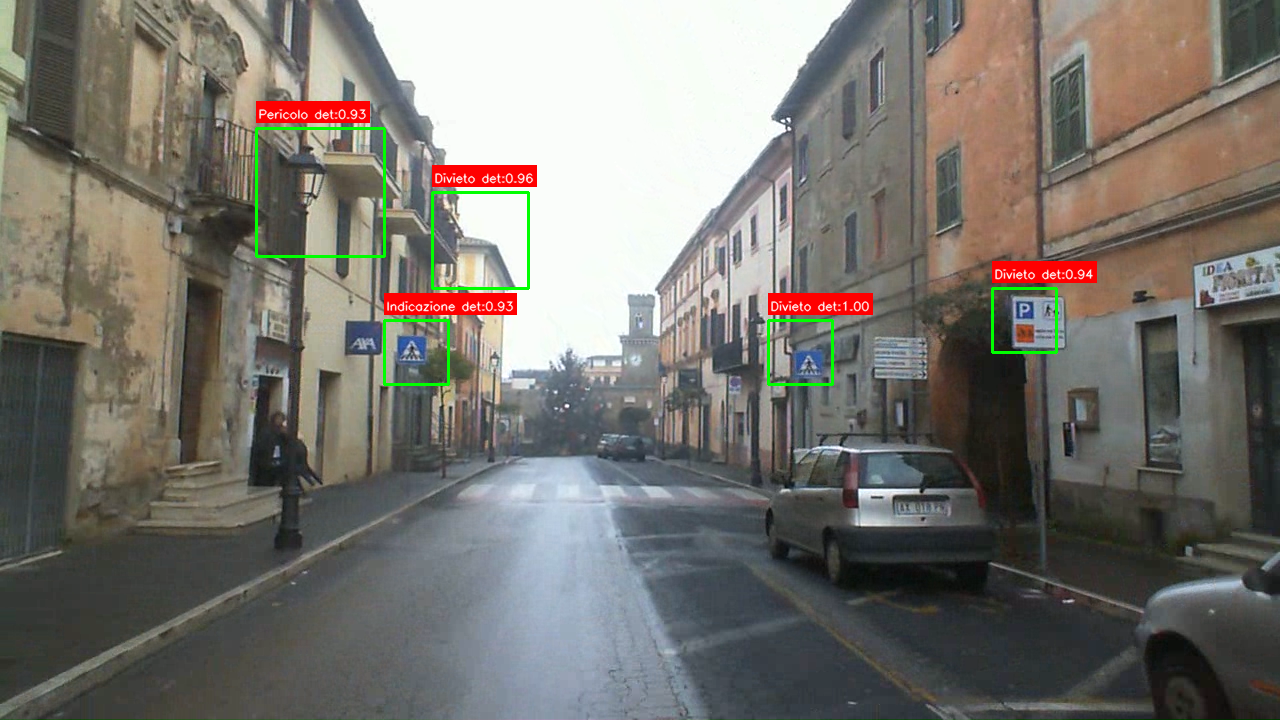
\includegraphics[width=0.9\linewidth]{Codice/test2_div.png}
    \caption{Divisione}
\end{subfigure}\hfill
\begin{subfigure}[t]{0.50\textwidth}
    \centering
    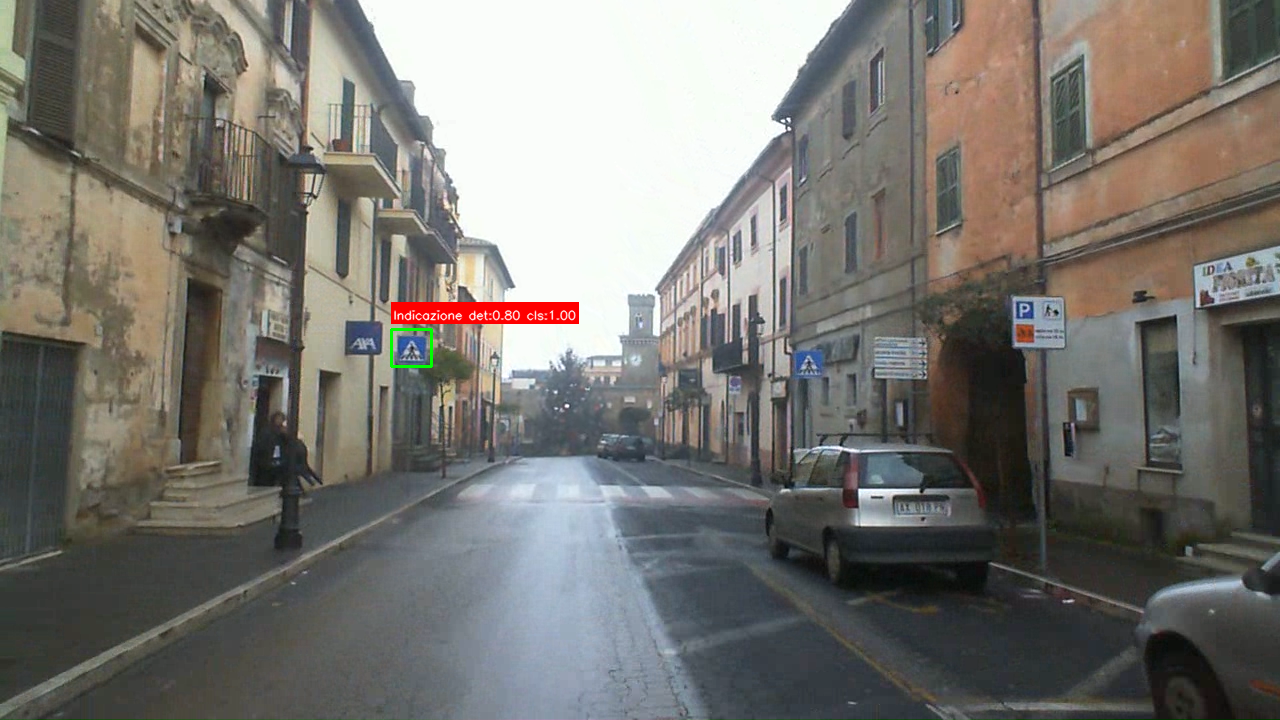
\includegraphics[width=0.9\linewidth]{Codice/test2_yolo.png}
    \caption{YOLO}
\end{subfigure}
\caption{Confronto tra i metodi di divisione e YOLO su un'immagine del dataset di test.}
\label{fig:test1}
\end{figure}

Per quanto riguarda invece il caso in cui viene usata un'immagine campione casuale presa online (Figura \ref{fig:test2}), possiamo notare che \textbf{YOLO} si è comportato meglio rispetto all'algoritmo di \textbf{divisione}, poiché quest'ultimo ha eseguito dei tagli che talvolta risultavano superflui.

\begin{figure}[htbp]
\centering
\begin{subfigure}[t]{0.33\textwidth}
    \centering
    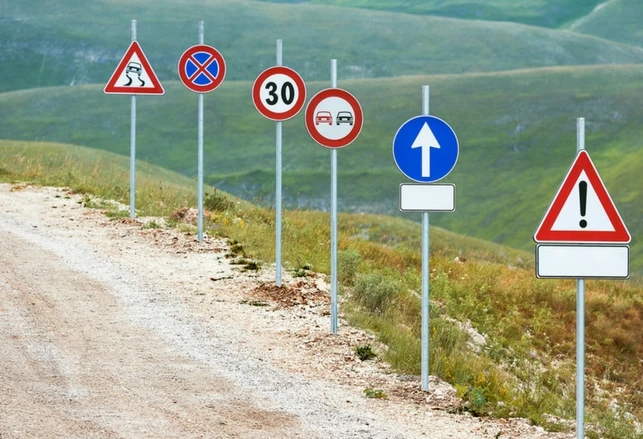
\includegraphics[width=0.9\linewidth]{Codice/test1.png}
    \caption{Immagine originale}
\end{subfigure}\hfill
\begin{subfigure}[t]{0.33\textwidth}
    \centering
    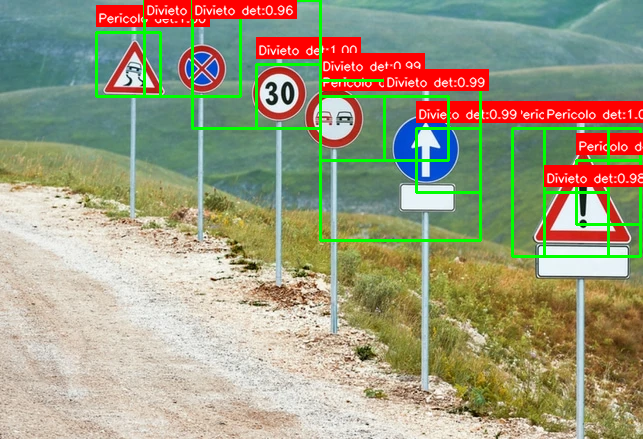
\includegraphics[width=0.9\linewidth]{Codice/test_div1.png}
    \caption{Divisione}
\end{subfigure}\hfill
\begin{subfigure}[t]{0.33\textwidth}
    \centering
    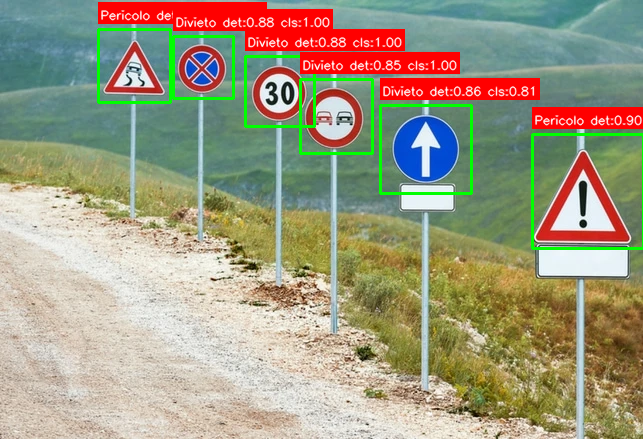
\includegraphics[width=0.9\linewidth]{Codice/test_yolo1.png}
    \caption{YOLO}
\end{subfigure}
\caption{Confronto tra i metodi di divisione e YOLO su un'immagine casuale.}
\label{fig:test2}
\end{figure}

In sintesi, nessuno dei due metodi si è rivelato perfetto nell'analisi di un contesto reale, ma entrambi possono essere utilizzati come punto di partenza per comprendere come procedere.

%\section{Uso quotidiano}
Nel notebook \textit{Result} è presente una seconda parte dopo il titolo \textbf{Uso Quotidiano} dove si utilizza la rete MiniAlexNetV2 con immagini reali (immagini prese dalla raccolta di test), in cui non si ha solo l'immagine del segnale ma si punta a ricnoscere il segnale in un contesto cidattino, per fare ciò ci si è posti il problema di come isolare la singola immagine del segnale stradale rispetto al contesto, per eseguire questa ricerca si sono usati 2 processi.
\begin{itemize}
    \item \textbf{Divisione in sottoimmagini:} Consiste nel suddividere l'immagine in tante piccole sotto immagini e poi per ognuna verificare cosa essa sia;
    \item \textbf{Uso di Yolo:} Uso di uno strumento che permette di ritagliare l'immagine per poter già verificare le sezioni migliori dell'immagini in cui sono presenti delle porzioni di immagini che sono candidabili per essere catalogate;
\end{itemize}

\subsection{Divisione in sottoimmagini}
L'uso dell'immagine in sottoimmagini all'inizio è sembrata l'idea migliore perchè era di facile operatività e di facile utilizzo, ma ha presentato scarsi risultati sia in terminni di velocità sia in termini di affidabilità.
Il motivo di questi scarsi risultati sono, per la velocità il fatto che l'immagine andrebbe tagliata pezzo per pezzo e questo causa una certa lentezza di calcolo, mentre per quanto riguarda il problema dei risultati esso è dovuto al fatto che il dataset non è abbastanza grande per poter analizzare tutti i casi possibili, se si avesse usato un dataset più grande possibilmente si poteva ottenere un risultato migliore.

\section{Conclusione}
I risultati ottenuti indicano che il modello proposto è in grado di affrontare efficacemente il compito assegnato, pur lasciando spazio a ulteriori miglioramenti. In prospettiva, si suggerisce di:
\begin{itemize}
  \item Aumentare quantità e diversità dei dati di addestramento, così da migliorare la capacità di generalizzazione della rete.
  
  \item Sperimentare architetture neurali alternative, al fine di individuare quella più adatta al riconoscimento dei segnali stradali.
  
  \item Rafforzare l'uso di tecniche di regolarizzazione per ridurre l'\textit{overfitting} e limitare l'eccessivo adattamento ai dati di addestramento.
  
  \item Ottimizzare gli \textit{iperparametri} (ad esempio tasso di apprendimento e dimensione del batch) per massimizzare le prestazioni del modello.
  
  \item Valutare la quantizzazione dei pesi per ridurre la complessità del modello mantenendo un livello di accuratezza adeguato.
  
  \item Analizzare le attivazioni nei diversi strati della rete per approfondire la comprensione del processo di apprendimento.
\end{itemize}

In sintesi, il lavoro svolto costituisce una base solida per sviluppi successivi nel riconoscimento dei segnali stradali mediante modelli di \textit{machine learning}. L'iterazione sperimentale e l'esplorazione di nuove soluzioni restano elementi centrali per affrontare scenari sempre più complessi. Una possibile evoluzione applicativa consiste nel passaggio dalla classificazione per macrocategorie all'identificazione del singolo segnale.


\begin{thebibliography}{2}
    \bibitem{FR22}
    \emph{S. Battiato, G. Signorello, G.M. Farinella, F. Ragusa, A. Furnari. Ego-ch: Dataset and fundamental tasks for visitors behavioral understanding using egocentric vision. 2019.}

    \bibitem{FR23}
    \emph{G.M Farinella, A. Furnari. Diapositive del corso di Machine Learning anno 2022/2023.}
\end{thebibliography}
    

\end{document}
